\documentclass[12pt, titlepage]{article}
\newcommand{\famname}{CFS} % PUT YOUR PROGRAM NAME HERE
\usepackage{booktabs}
\usepackage{tabularx}
\usepackage{hyperref}
\hypersetup{
    colorlinks,
    citecolor=black,
    filecolor=black,
    linkcolor=red,
    urlcolor=blue
}
\usepackage[round]{natbib}
\usepackage{xcolor}
\usepackage{amsmath, mathtools}
\usepackage{amsfonts}
\usepackage{amssymb}
\usepackage{graphicx}
\usepackage{colortbl}
\usepackage{xr}
\usepackage{hyperref}
\usepackage{longtable}
\usepackage{xfrac}
\usepackage{float}
\usepackage{siunitx}
\usepackage{caption}
\usepackage{pdflscape}
\usepackage{afterpage}
\usepackage{comment}
%% Comments

\usepackage{color}

\newif\ifcomments\commentstrue

\ifcomments
\newcommand{\authornote}[3]{\textcolor{#1}{[#3 ---#2]}}
\newcommand{\todo}[1]{\textcolor{red}{[TODO: #1]}}
\else
\newcommand{\authornote}[3]{}
\newcommand{\todo}[1]{}
\fi

\newcommand{\wss}[1]{\authornote{blue}{SS}{#1}}
\newcommand{\an}[1]{\authornote{magenta}{Malavika}{#1}}



\usepackage{titlesec}


\begin{document}

\title{CFS: System Verification and Validation Plan} 
\author{Malavika Srinivasan}
\date{\today}
	
\maketitle

\pagenumbering{roman}


\section{Revision History}

\begin{tabularx}{\textwidth}{p{3cm}p{2cm}X}
\toprule {\bf Date} & {\bf Version} & {\bf Notes}\\
\midrule
Oct 16, 2018 & 1.0 & First draft by Malavika\\
\bottomrule
\end{tabularx}

~\newpage

\section{Symbols, Abbreviations and Acronyms}

\renewcommand{\arraystretch}{1.2}
\begin{tabular}{l l} 
  \toprule		
  \textbf{symbol} & \textbf{description}\\
  \midrule 
  T & Test\\
  \bottomrule
\end{tabular}\\
\\
Also see the table of symbols in CA at: \url{https://github.com/Malavika-Srinivasan/CAS741/tree/master/docs/SRS/CA.pdf}{Table of Symbols}\\


\newpage

\tableofcontents

\listoftables

\listoffigures

\newpage

\pagenumbering{arabic}

Verification and Validation .....\ms{Needs more explanations}



This document explains the verification and validation plan to improve the quality of \famname{}. There are several standards available for software quality and according to the quality model of ISO 9126,  software quality is described as a structured set of characteristics namely - Functional suitability, Performance, efficiency, Compatibility, Usability,  Reliability, Security, Maintainability and Portability ~\cite{ISO25000}.

Here we restrict ourselves to Functional suitability, Maintainability and portability. 


\section{General Information}

This section explains the summary of what is being tested in this document, the objectives of this document and references for this document. 


\subsection{Summary}

This document will summarize the plan for verification and validation of \famname{} for compliance with the requirements specified in the CA document. 
The goal statement as found in CA document is presented below.
\\
\\
\noindent ``Given the set of data points, the choice of software from \famname{} and the variabilities of the software the \famname{} should:

\begin{enumerate}
	
	\item compute the parameters of the curve which is the best possible fit through the set of data points.	''
\end{enumerate}

The process explained in the goal statement is called curve fitting. There different choices like regression, interpolation and smoothing. This is explained better in the Figure \ref{Fig_CurveFitEg}.

\begin{figure}[h!]
	\begin{center}
		%rotatebox{-90}
		{
			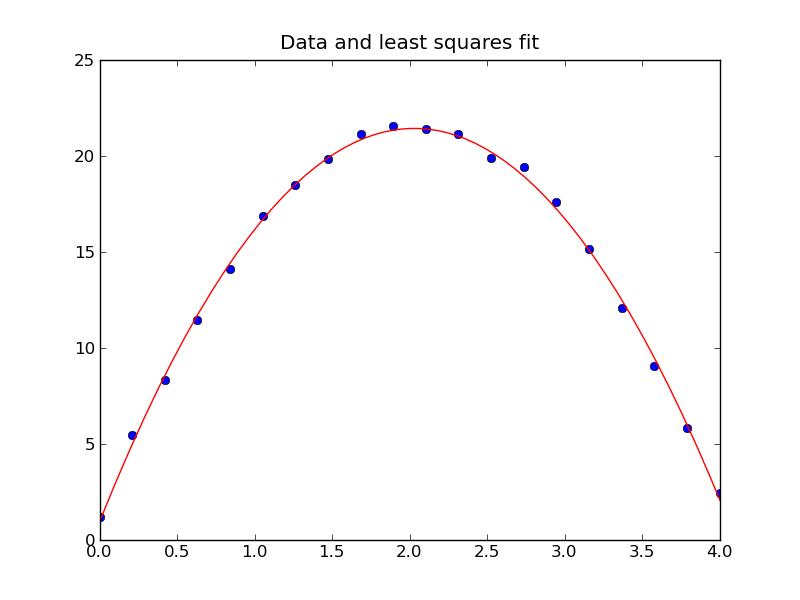
\includegraphics[width=0.5\textwidth]{lstsq11.png}
		}
		\caption{\label{Fig_CurveFitEg} Typical example of a curve fitting process}
	\end{center}
\end{figure}

\wss{Say what software is being tested.  Give its name and a brief overview of
  its general functions.}

\subsection{Objectives}

The goal of verifying and validating is to increase improve the quality of the \famname{} and obtain confidence in the software implementation. The qualities which are important concerning \famname{} are correctness(Functional suitability), maintainability, re-usability, portability. The definitions of the above mentioned qualities are explained below.

\subsubsection {Functional Suitability}

This characteristic represents the degree to which a product or system provides
functions that meet stated and implied needs when used under specified
conditions. It can be further characterized into completeness, correctness and
appropriateness.
\paragraph{Correctness }
The degree to which a product or system provides the correct results with the
needed degree of precision.

\subsubsection{Maintainability}
This characteristic represents the degree of effectiveness and efficiency with
which a product or system can be modified to improve it, correct it or adapt it
to changes in the environment, and in requirements. Reusability is an important characteristic of maintainability.
\paragraph{Reusability}
The degree to which an asset can be used in more than one system, or in
building other assets.

\subsubsection{Portability}
The degree of effectiveness and efficiency with which a system, product or
component can be transferred from one hardware, software or other operational
or usage environment to another. 

\wss{State what is intended to be accomplished.  The objective will be around
  the qualities that are most important for your project.  You might have
  something like: ``build confidence in the software correctness,''
  ``demonstrate adequate usability.'' etc.  You won't list all of the qualities,
  just those that are most important.}

\subsection{References}

Throughout this document, we refer to the terminologies that have been already explained in the CA document for Program \famname{}.
\wss{Reference relevant documentation.  This will definitely include your SRS}

\section{Plan}
	
\subsection{Verification and Validation Team}

\begin{enumerate}
	\item Malavika srinivasan
\end{enumerate}



\wss{Probably just you.  :-)}

\subsection{SRS Verification Plan}

The CA document for \famname{} will be reviewed by Dr.Spencer Smith and my classmate Mr.Robert White.

\wss{List any approaches you intend to use for SRS verification.  This may just
  be ad hoc feedback from reviewers, like your classmates, or you may have
  something more rigorous/systematic in mind..}

\subsection{Design Verification Plan}

My design will be verified with the help of my supervisor Dr.Spencer Smith and my classmates Ms.Jennifer Garner and Mr.Brooks MacLachlan.
\wss{Plans for design verification}

\subsection{Implementation Verification Plan}


My implementation will be verified by the tests listed in this document and the unitVnVplan document. My classmate Ms.Vajiheh Motamer will help me verify the document.	
\wss{You should at least point to the tests listed in this document and the unit
  testing plan.}

\subsection{Software Validation Plan}

\ms{I am a little confused about this section. I am not sure if this is relevant for my general purpose tool. I have other softwares from which I can do parallel testing but not an external data for vaidation. Needs to be confirmed.}

\wss{If there is any external data that can be used for validation, you should
  point to it here.  If there are no plans for validation, you should state that
  here.}

\section{System Test Description}

System testing is a process in which only the overall working of the system. The instance models in CA document will be tested here. This does not test the inidividual units or modules of the system. It is a black box testing approach.
	
\subsection{Tests for Functional Requirements}

\wss{Subsets of the tests may be in related, so this section is divided into
  different areas.  If there are no identifiable subsets for the tests, this
  level of document structure can be removed.}

\subsubsection{Interpolation Testing}
\ms{Not sure if I can have an area for interpolation and regression, but I have it here as a place holder}		
%#######################################################
\paragraph{Testcase for Polynomial interpolation}

\begin{enumerate}

\item{\textbf{T1: Simple example of monomial interpolation} \\}

Control: Automatic \ms{Pytest or robot framework}
					
Initial State: NA
					
Input: Data points (-2,-9), (-1, -15), (0,-5), (1,-3), (2,39)
					
Output: (−5, 4, −7, 2, 3) (coefficients of the increasing powers of x, starting from $x^{0}$ )
					
How test will be performed: \ms{I am not sure what goes here}


%#######################################################
					
\item{T2: Simple example of Lagrange's interpolation \\}

Control: Manual versus Automatic
					
Initial State:NA 
					
Input: Data points (4.1168, 0.213631), (4.19236,0.214232), (4.20967, 0.21441, 4.46908, 0.218788)
					
Output: (0.871839, -0.386008, 0.0695519, -0.00355245) (coefficients of the increasing powers of x, starting from $x^{0}$ )
					
How test will be performed: \ms{I am not sure what goes here}

%#######################################################

\item{T3: Simple example of Newton interpolation \\}

Control: Automatic \ms{Pytest or robot framework}

Initial State: NA

Input: Data points (0,1), (1,2.25), (2,3.75), (3,4.25)

Output: 1, 1.25, 0.125, -0.20833 (coefficients of the increasing powers of (x - $x_i$, starting from $(x - x_i)^{0}$ where i = 0,1,2 )

How test will be performed: \ms{I am not sure what goes here}



%#######################################################

\paragraph{Testcase for Piecewise Polynomial interpolation}

\item{T4: Simple example of Hermite Cubic interpolation \\}

Control: Automatic \ms{Pytest or robot framework}

Initial State: NA

Input: Data points (0,1), (1,2.25), (2,3.75), (3,4.25)

Output: 1, 1.25, 0.125, -0.20833 (coefficients of the increasing powers of (x - $x_i$, starting from $(x - x_i)^{0}$ where i = 0,1,2 )

How test will be performed: \ms{I am not sure what goes here}




%#######################################################


\item{T5: Simple example of BSpline interpolation \\}

Control: Automatic \ms{Pytest or robot framework}

Initial State: NA

Input: Data points (0,1), (1,2.25), (2,3.75), (3,4.25)

Output: 1, 1.25, 0.125, -0.20833 (coefficients of the increasing powers of (x - $x_i$, starting from $(x - x_i)^{0}$ where i = 0,1,2 )

How test will be performed: \ms{I am not sure what goes here}



%#######################################################
%#######################################################
%#######################################################

\subsubsection{Regression}

\item{T6: Simple example of regression using normal equations \\}

Control: Automatic \ms{Pytest or robot framework}

Initial State: NA

Input: Data points 

Output: 

How test will be performed: \ms{I am not sure what goes here}




\item{T7: Simple example of regression using Augmented system\\}

Control: Automatic \ms{Pytest or robot framework}

Initial State: NA

Input: Data points 

Output: 

How test will be performed: \ms{I am not sure what goes here}




\item{T8: Simple example of regression using Orthogonal transformations\\}

Control: Automatic \ms{Pytest or robot framework}

Initial State: NA

Input: Data points 

Output: 

How test will be performed: \ms{I am not sure what goes here}

%#######################################################
%#######################################################
%#######################################################
%#######################################################
%#######################################################
%#######################################################

\end{enumerate}
\subsection{Tests for Nonfunctional Requirements}

\subsubsection{Correctness}
		
\paragraph{Parallel testing}

\begin{enumerate}

\item{T9: Parallel Testing\\}


Type: 
					
Initial State: 
					
Input/Condition: 
					
Output/Result: 
					
How test will be performed: 
				
				
				
%#######################################################				
\subsubsection{Maintainability}				
					
\item{T9: \\}

Type: Functional, Dynamic, Manual, Static etc.
					
Initial State: 
					
Input: 
					
Output: 
					
How test will be performed: 


%#######################################################


\end{enumerate}

\subsubsection{Area of Testing2}

...

\subsection{Traceability Between Test Cases and Requirements}

The following table shows the traceability mapping for test cases, instance models and the requirements. \ms{I feel adding instance models here makes the table clearer. Needs to be discussed}

\begin{table} [H]
	\caption{Requirements Traceability Matrix}
	\label{Table:Table_Traceability}  
	\begin{tabular}{|c|p{5cm}|p{5cm}|}
		\hline	
		\textbf{Test Number} & \textbf{Instance Models} & \textbf{CA Requirements}\\
		\hline 
		T1& IM3, IM1& R5, R6\\ \hline
		T2& IM4, IM1& R5, R6\\ \hline
		T3& IM5, IM1& R5, R6\\ \hline
		T4& IM6, IM1& R5, R7\\ \hline
		T5& IM7, IM1& R5, R7\\ \hline
		T6& IM8, IM2& R5, R8\\ \hline
		T7& IM9, IM2& R5, R8\\ \hline
		T8& IM10,IM2& R5, R8\\ \hline
		
	\end{tabular}\\
\end{table}




\section{Static Verification Techniques}

\wss{In this section give the details of any plans for static verification of
  the implementation.  Potential techniques include code walkthroughs, code
  inspection, static analyzers, etc.}
				
\bibliographystyle{plainnat}

\bibliography{SRS}

\newpage

\section{Appendix}

This is where you can place additional information.

\subsection{Symbolic Parameters}

The definition of the test cases will call for SYMBOLIC\_CONSTANTS.
Their values are defined in this section for easy maintenance.

\subsection{Usability Survey Questions?}

\wss{This is a section that would be appropriate for some projects.}

\end{document}